\chapter{Save Page}

The Save Page is used to save track data from the Internal Sequencer, Machinedrum or AnalogFour to  specific slots in the current row of the focused Grid.\\
\\
There are three different save modes available:
\begin{itemize}
    \item SEQ: Save internal sequencer data and MD sound data.
    \item MD: Copy MD Sequencer data. Save MD sequencer data and MD sound data. Internal sequencer data is not saved.
    \item MERGE: Merge MD Sequencer data with internal sequencer. Save sequencer data and MD sound data.
\end{itemize}
\textit{For technical reasons, MD and MERGE modes are only available when the sequencer playback is stopped.}
\\
\\The Save page is also used to save A4 tracks. When an A4 track is saved, the Sound Settings for the chosen track together with the internal sequencer data are stored together. Save mode has no effect here.

%\fbox{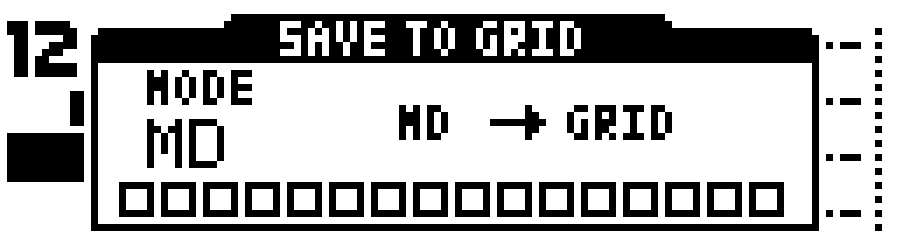
\includegraphics[scale=.40]{save_page.png}}\\

\screenshot{save_to_grid.png}

\textit{The Save Page is accessible from the GridPage by pressing the  \textbf{[Save]} function button.}

\encodersbuttons{Mode}{--}{--}{--}{cancels the save.}{--}{--}{Group Select}

\section{Saving Individual Tracks}
The Save Page uses the Trigger Interface to specify which tracks are to be saved. Pressing multiple trigger buttons on the MD and then releasing them will cause the selected tracks to be stored in the corresponding slots of the current row.
\section{Grid Toggle}
The \textbf{[ Shift 1 ]} button can be used to toggle between Grid A or Grid B.\\\\
It is possible to simultaneously save a collection of tracks from both Grids A and B. 
\begin{itemize}
\item First select the tracks from one grid by pressing and holding the corresponding triggers.
\item Tap \textbf{[ Shift 1 ]} to switch grids
\item Release the trig selection
\item Select tracks from alternate grid by pressing and holding the corresponding triggers. 
\item Finally release the second grid selection to confirm the action. 
\end{itemize}

\section{Save Track Groups:}
When in the Save or Load Page, holding the [ Shift 2 ] button now opens a Group Select menu,
allowing you to load or save all tracks corresponding to a group. An entire row/pattern across both grids A+B can be saved this way.\\
\\
There are four groups:
\begin{enumerate}
    \item MIDI Device 1 (MD)
    \item MIDI Device 2 (A4/MNM/Generic)
    \item FX (MDFX + LFOTrack + RouteTrack)
    \item TP (Tempo)
\end{enumerate}
The groups can be enabled/disabled using the MD's trigger interface.\\
\\
Releasing [ Shift 2 ] will save/load tracks corresponding to the active groups.


